\chapter*{Opis aplikacji}
%Trochę o poruszaniu, spline'ach i narzędziu do nich (screen narzedzia)
%Opisać co to scenariusze i narzędzie do nich (screen narzedzia)
%Albo może te rzeczy w następnym rozdziale
Po uruchomieniu aplikacji użytkownikowi najpierw ukazuje się ekran ładowania (przedstawiony na rysunku~\ref{fig:splash}), a następnie menu główne (widoczne na rysunku~\ref{fig:ap1}).
\begin{figure}[h]
	\centering
	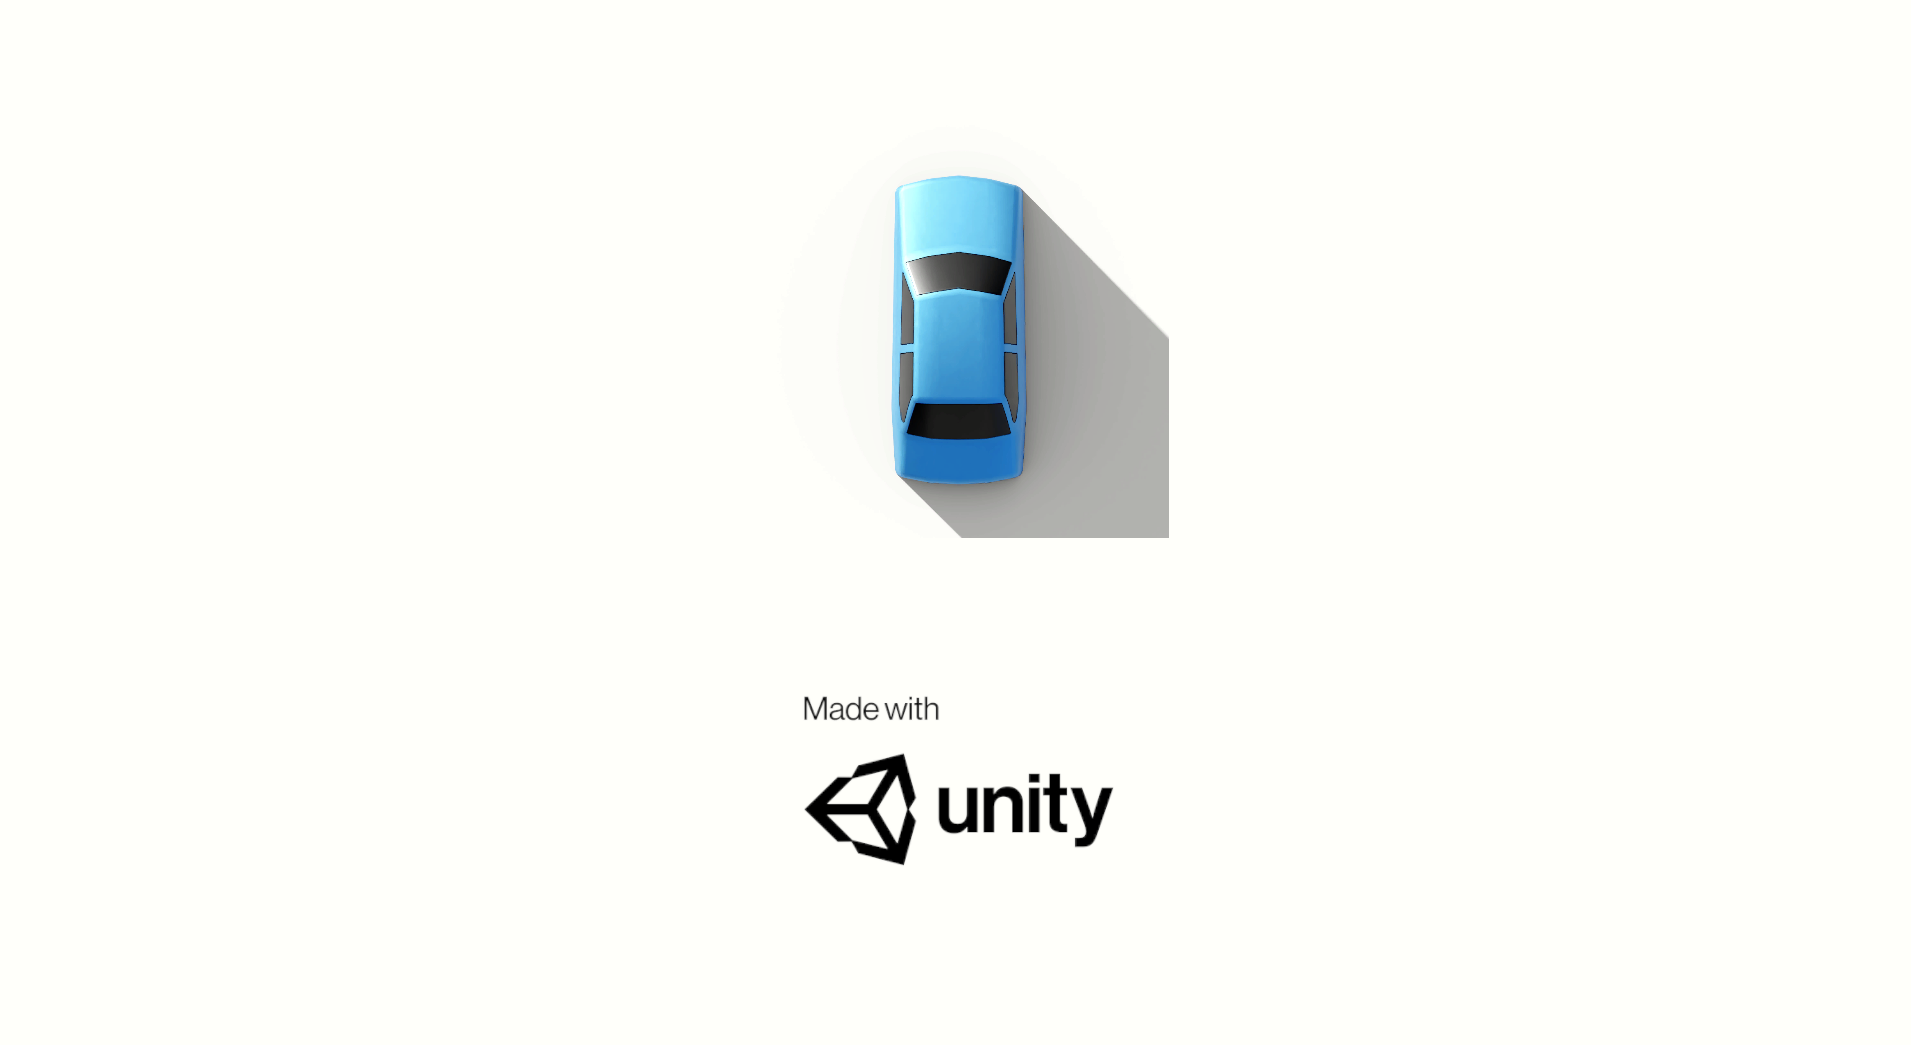
\includegraphics[width=1\linewidth]{splash}
	\caption[Ekran ładowania aplikacji]{Ekran ładowania aplikacji}
	\label{fig:splash}
\end{figure}

\section*{Menu główne}
W górnej części menu znajdują się pola liczbowe, do których użytkownik może wpisać ustawienia symulacji oraz algorytmu ewolucyjnego. Może też skorzystać z ustawień domyślnych. \\Dostępne ustawienia symulacji to:
\begin{itemize}
	\item Prędkość symulacji -- jest to mnożnik prędkości symulowania ruchu drogowego. Przy ustawieniu 1x przeliczane jest 30 kroków symulacji na sekundę. Jedynym górnym ograniczeniem tego ustawienia jest moc obliczeniowa procesora. Domyślna wartość to 100x. \\
	\item Liczba samochodów na pasie -- jest to liczba samochodów, które wjadą na każdy pas ruchu (pasy są widoczne w lewym dolnym rogu rysunku~\ref{fig:ap1}). Domyślna wartość to 20.\\
\end{itemize}
Ustawienia algorytmu ewolucyjnego przedstawiają się następująco:
\begin{itemize}
	\item Populacja pokolenia -- liczba osobników w każdym pokoleniu (stała $n$ w funkcji~\ref{fitness} w poprzednim rozdziale).\\
	\item Liczba pokoleń -- liczba pokoleń, po których proces uczenia ma zostać przerwany. Oprócz tego wpływa na współczynnik mutacji (stała $g$ w funkcji~\ref{mutRate} w poprzednim rozdziale).\\
	\item Długość kroku scenariusza -- zakres w jakim muszą się mieścić wartości parametrów osobników, a więc długości kroków scenariusza.\\
	\item Maksymalny współczynnik mutacji -- stała $m$ w funkcji~\ref{mutRate} w poprzednim rozdziale.\\
\end{itemize}
\begin{figure}[h]
	\centering
	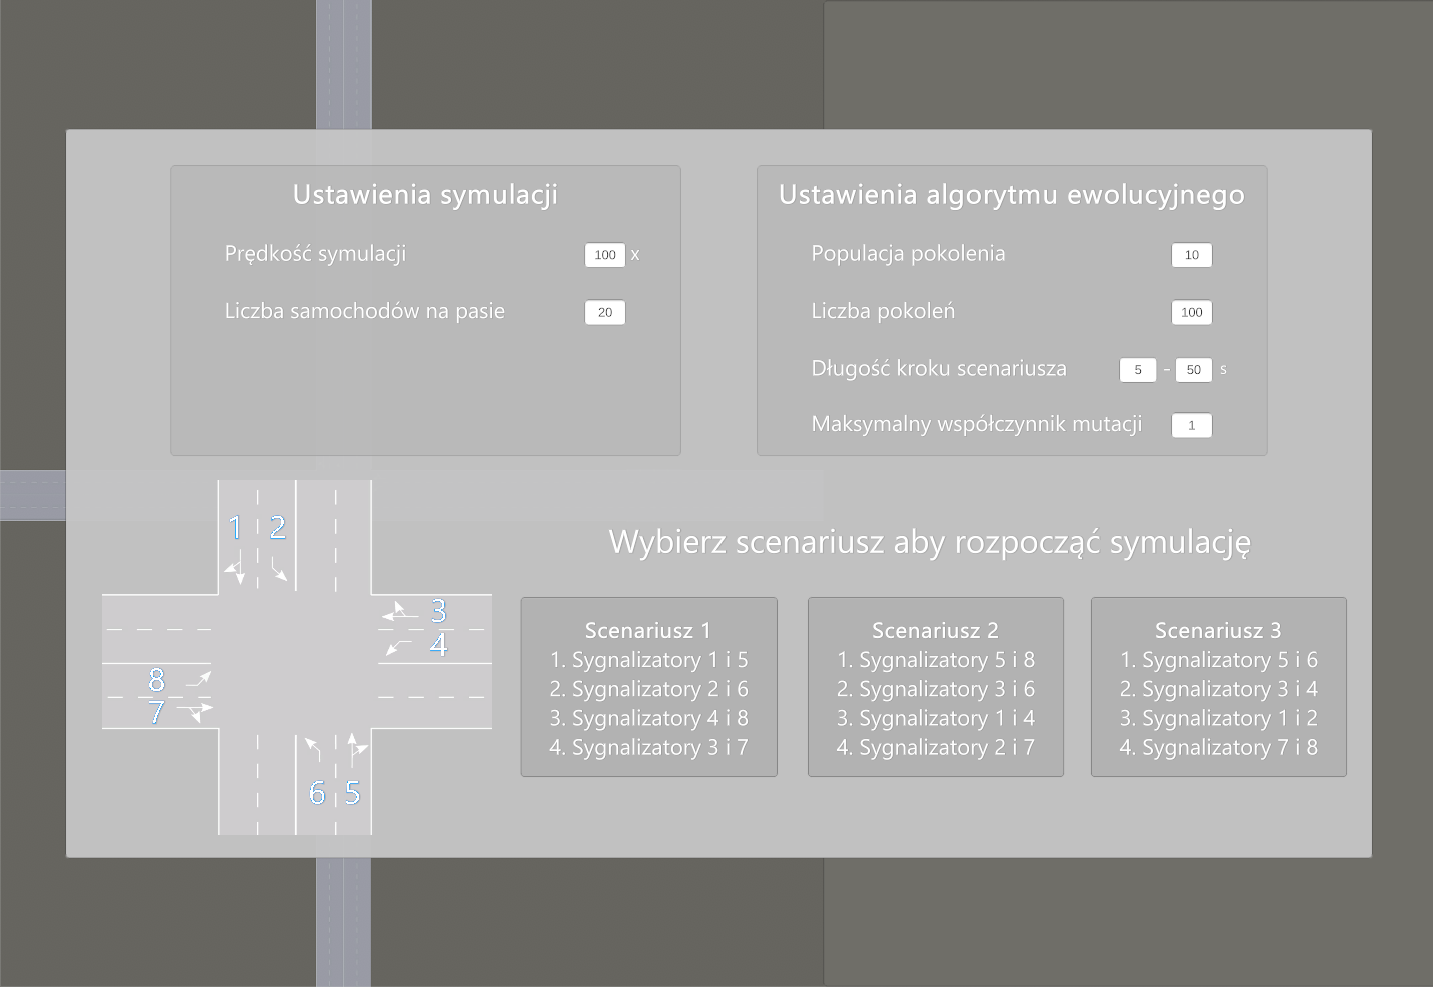
\includegraphics[width=1\linewidth]{ap1}
	\caption[Menu główne aplikacji]{Menu główne aplikacji}
	\label{fig:ap1}
\end{figure}
Po wybraniu ustawień użytkownik musi wybrać scenariusz. Jest to sekwencja sygnalizatorów, które będą zielone w określonym kroku scenariusza. W lewym dolnym rogu menu (na rysunku~\ref{fig:ap1}) widoczny jest schemat z ponumerowanymi sygnalizatorami, mający na celu ułatwienie użytkownikowi zrozumienia różnicy między scenariuszami. 
\section*{Scenariusz} Na przykładzie Scenariusza~1 widocznego w menu: podczas pierwszego kroku scenariusza zielone będą sygnalizatory nr 1 i 5 (oznaczone na schemacie po lewej), zaś pozostałe będą czerwone. Po przejściu do drugiego kroku zielone będą sygnalizatory nr 2 i 6, podczas gdy pozostałe będą czerwone. Analogicznie w kolejnych krokach scenariusza. Długość każdego z tych kroków opisuje obecnie symulowany osobnik.
\section*{Przebieg uczenia i symulacji ruchu}
Po wybraniu scenariusza rozpoczyna się proces uczenia. Aplikację podczas tego procesu przedstawia rysunek~\ref{fig:ap2}. Lewa część ekranu prezentuje postęp symulacji ruchu drogowego z zastosowaniem parametrów świateł obecnie symulowanego osobnika.
\begin{figure}[h]
	\centering
	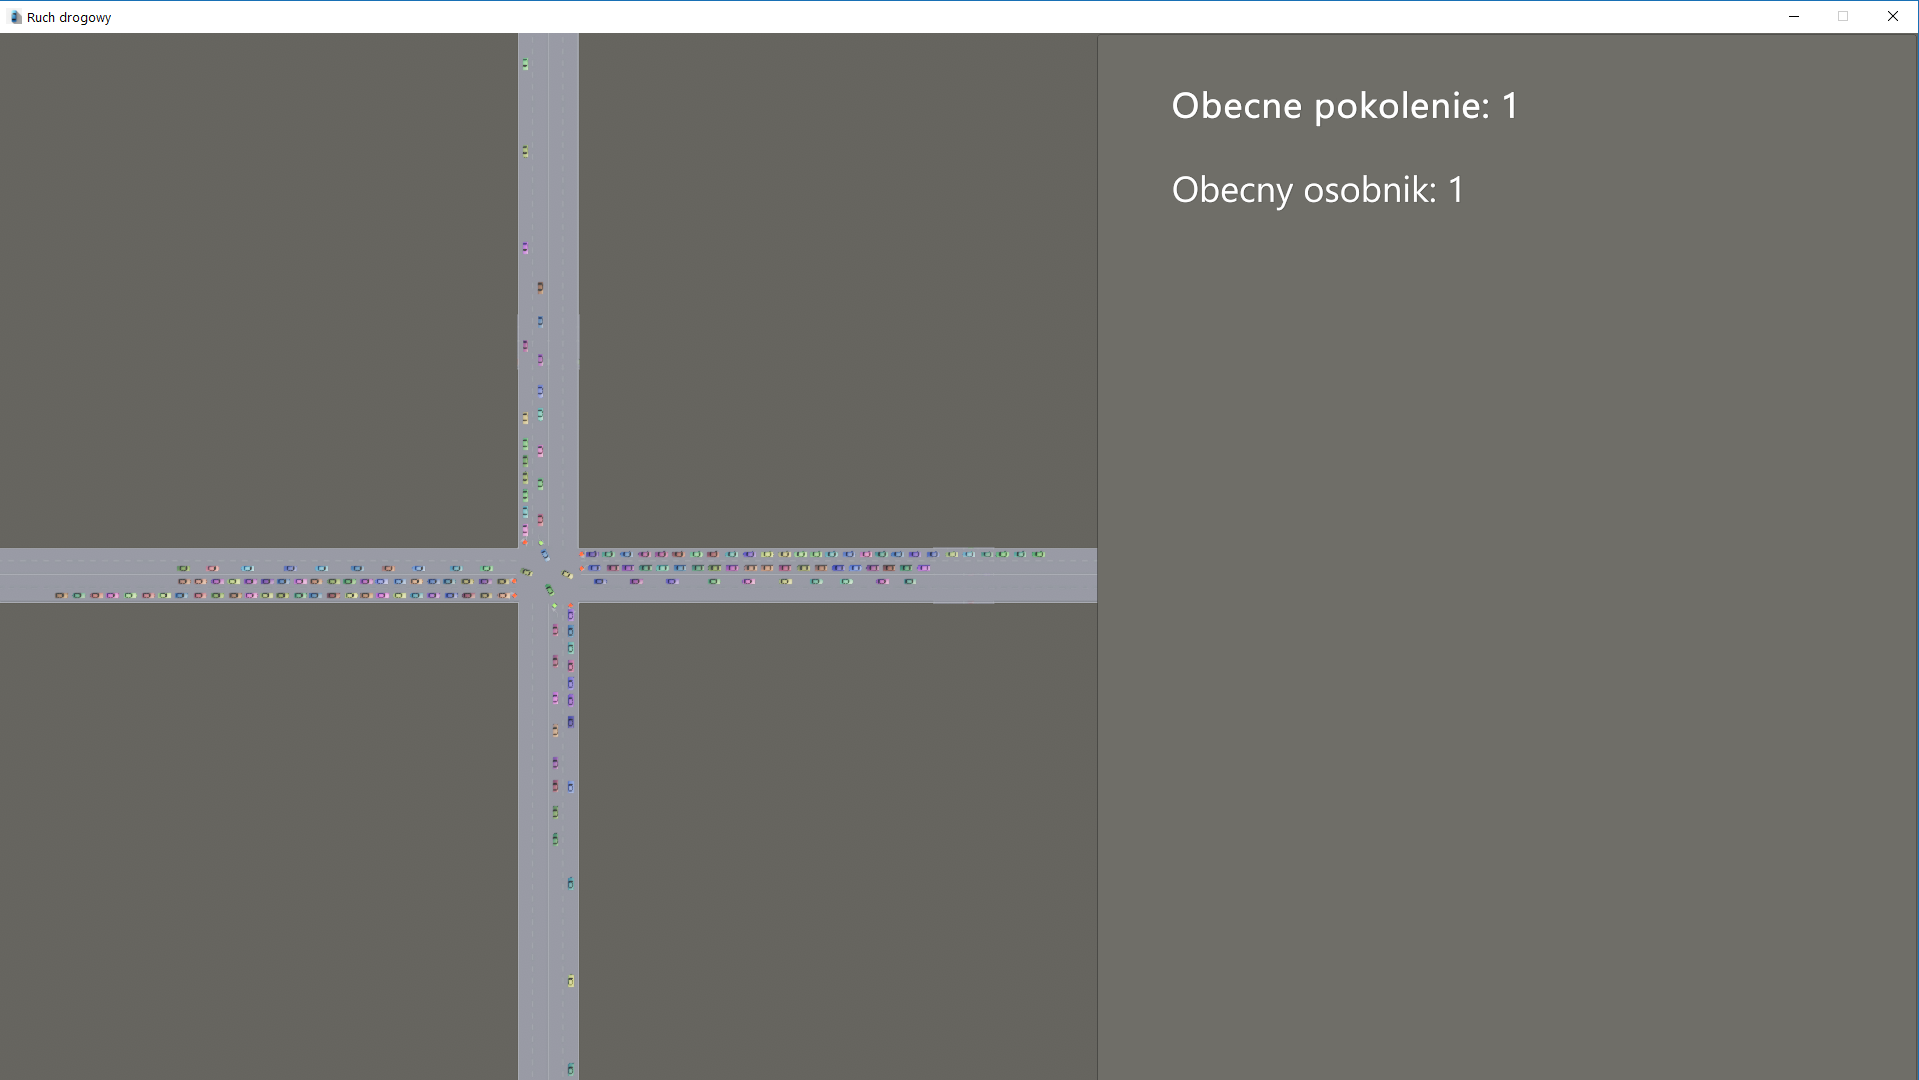
\includegraphics[width=1\linewidth]{ap2}
	\caption[Proces uczenia i symulacji ruchu]{Proces uczenia i symulacji ruchu}
	\label{fig:ap2}
\end{figure}


